\section{Eredmények}
A vizsgálatok menetének első része a szintetikus kísérleti adatok előállítása volt: Összeállítottunk egy idegsejtmodellt és ennek az adott modellparaméterek melletti áramlépcső stimulusra adott válaszfüggvényére (ami egy determinisztikus adathalmaz) egy zajmodellt (\ref{sec:noise}) raktunk, így szimulálva a kísérleti adatokat. Majd ezekre az adatokra végeztük el a paraméterbecslést. Ezzel a módszerrel meg tudjuk mondani az inferencia pontosságát adott típusú zajt feltételezve (és adott kísérleti protokoll mellett), mert ismerjük a kiinduló paramétereket.

Végül valódi mérési eredményekre is alkalmaztuk a módszereinket. Minden esetben passzív idegsejtmodellekkel dolgoztunk.

\subsection{Fehér zaj}
A következő pontokban összefoglaljuk a fehér zaj mellett kapott eredményeket.
\subsubsection{Egykompartmentumos modell egy változóval}
Az a kérdés, hogy passzív egykompartmentumos modell (\ref{sec:single-comp}) áramlépcső stimulusra adott feszültségválasza segítségével milyen pontosan tudjuk megbecsülni a kiindulási paramétereket (amikkel a szintetikus adatot előállítottuk) fehér zajt feltételezve, egyetlen változó paraméter mellett ($cm$). A zaj szórását nagyra $\sigma_{zaj} = 7$-re választottuk, ezzel a beállítással az adatok \ref{fig:white} ábra jobb oldalán látható módon néznek ki. A $cm$ paraméteren végzett inferencia eredménye a \ref{fig:wn1} ábrán látható.

Elvégeztünk 100 darab paraméterbecslést annak érdekében, hogy lássuk a módszer robusztusságát. A következő paraméterbeállításokkal futtattuk a becsléseket:
\begin{verbatim}
	cm = 1.
	gpas = 0.0001
	cm_start = 0.4
	cm_end = 1.6
	cm_num = 100
	cm_mean = 1.
	cm_sig = 0.2
	noise_sigma = 7
\end{verbatim}
Végeredményként ezek a statisztikák adódtak:

\begin{verbatim}
	(A) A becsült paraméter igazitól való távolsága átlagban: 0.0568
	(B) Az előbbi érték szórása: 0.043
	(C) A poszterior eloszlás maximuma (becsült paraméter), 
	    hányszorosa az igazi értékhez tartozó valószínűségnek átlagban: 2
	(D) Az előbbi érték szórása: 1.9
	(E) A poszterior eloszlás hányszor élesebb a prior eloszlásnál átlagban: 2.75
	(F) A felső érték szórása: 0.11	
\end{verbatim}
A (C) és (D) pont érdekes, azt mutatja, hogy nagy kiugrások lehetségesek. A statisztikák szemléltetése a \ref{fig:wn1-stat} ábrán látható. 


\begin{figure}[!htb]
	\centering
	\includegraphics[width=0.7\textwidth]{./fig/wn1/wn1.png}
	\caption[Egy kompartmentum, fehér zaj, egy paraméter eredmény]{Az inferencia eredménye $gpas = 0.0001$ és $\sigma_{zaj} = 7$ beállítások mellett a $cm$ változóra. Jól látható, hogy még hatalmas zaj mellett is szép a becslés. (A függőleges zöld vonal a $cm$ valódi értéke.)}
	\label{fig:wn1}
\end{figure}

\begin{figure}
	\hfill
	\subfloat[(A) pont]{{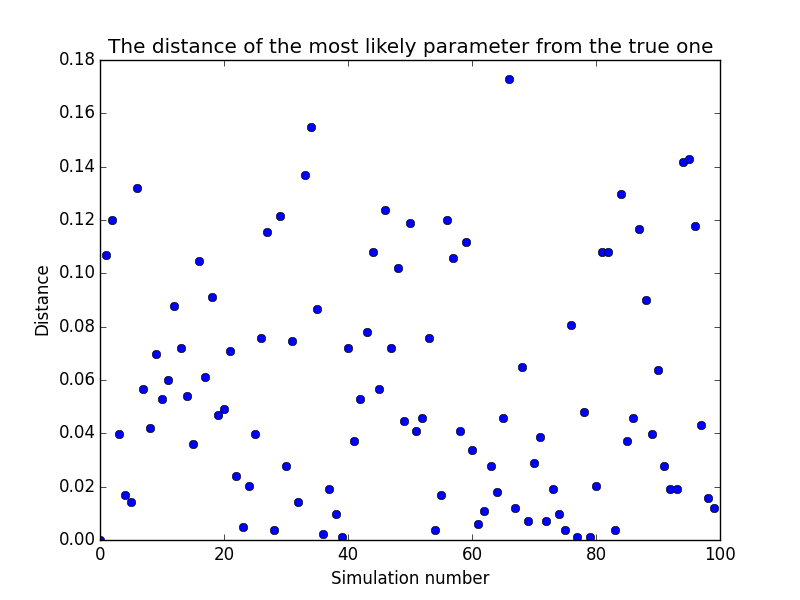
\includegraphics[width=0.49\textwidth]{./fig/wn1/dist200.png} }}%
	\hfill
	\subfloat[(C) pont]{{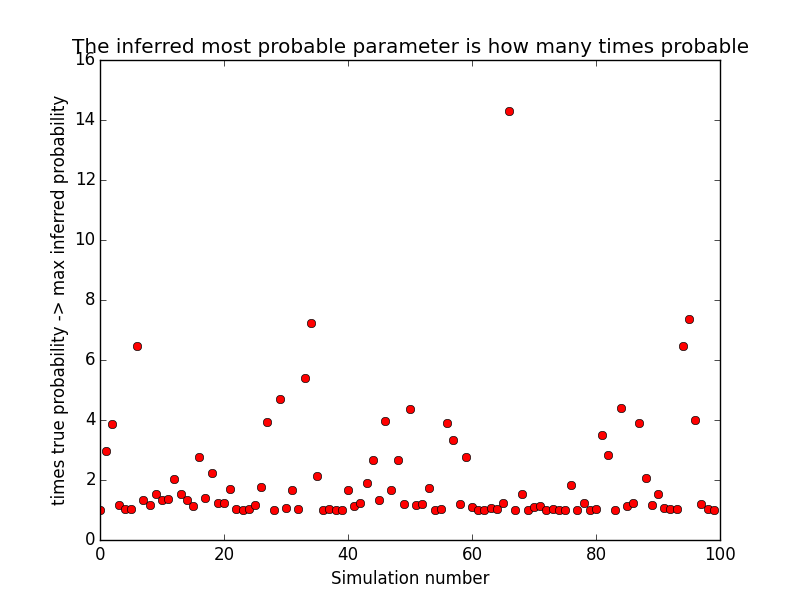
\includegraphics[width=0.49\textwidth]{./fig/wn1/p_times200.png} }}%
	\hfill
	\vfill
	\subfloat[(E) pont]{{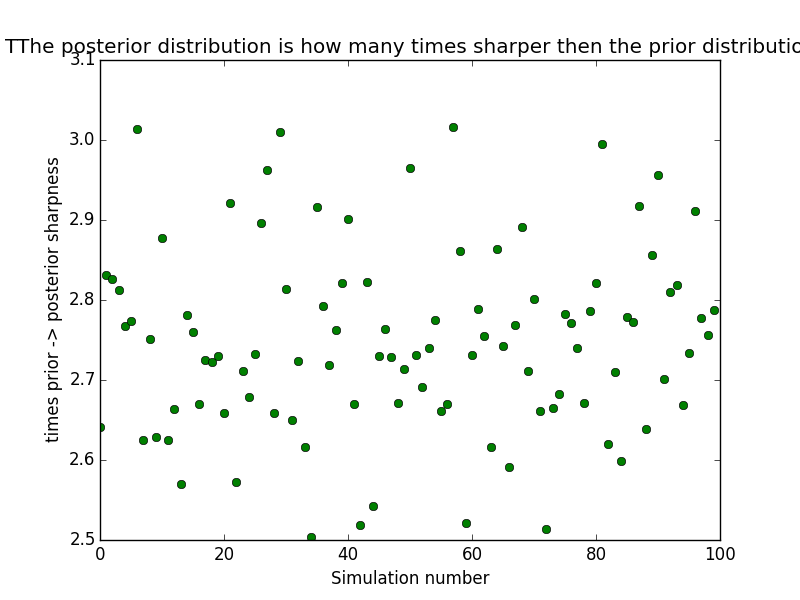
\includegraphics[width=0.5\textwidth]{./fig/wn1/sharp_times200.png} }}%
	\hfill
	\subfloat[Kiugró eset]{{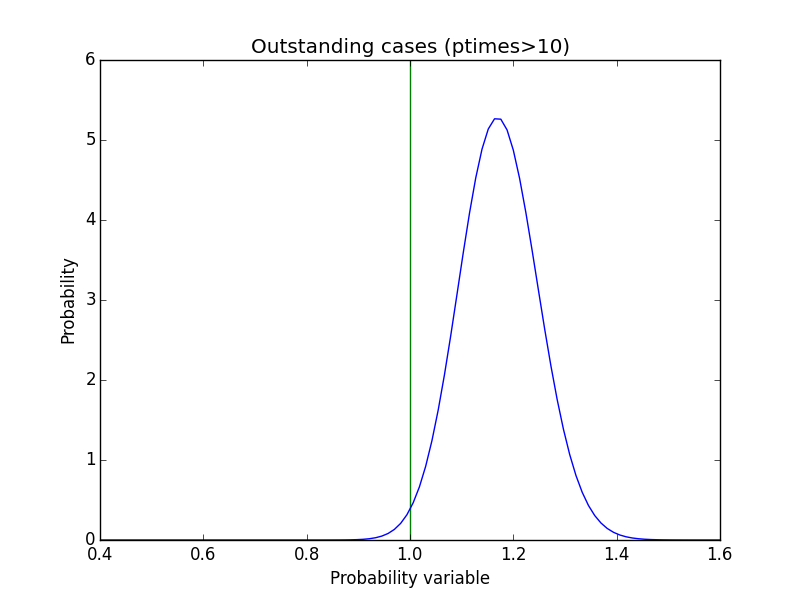
\includegraphics[width=0.5\textwidth]{./fig/wn1/outstanding100_81.png} }}%
	\caption[Egykompartmentum, fehér zaj, egy paraméter statisztika]{Az első három képen sorban az (A)(C)(E) statisztikák szemléltetése, az utolsón pedig egy kiugró eset látható.}%
	\label{fig:wn1-stat}
\end{figure}



\FloatBarrier
\subsubsection{Egykompartemntumos modell két változóval}
Ebben a részben azt vizsgáljuk, hogy a $cm$ paraméter becslését mennyire befolyásolja egy új változó paraméter jelenléte ($gpas$).
A \ref{fig:wn2} ábrán látható egy inferencia eredménye. Ebben az esetben is elvégeztük a 100 futtatásból álló elemzést két zaj esetén is. Az előző részben használt zajt alkalmazzuk, hogy aztán összehasonlíthassuk az eredményeket, valamint egy annál kisebb zajt (az elvárásoknak megfelelően azt tapasztaltuk, hogy a kisebb zaj esetén pontosabb eredményeket kapunk). A kapott eredmények:
\begin{verbatim}
(A) A becsült paraméter igazitól való távolsága átlagban: 0.053
(B) Az előbbi érték szórása: 0.039
(C) A poszterior eloszlás maximuma (becsült paraméter), 
hányszorosa az igazi értékhez tartozó valószínűségnek átlagban: 2.2
(D) Az előbbi érték szórása: 3.8
(E) A poszterior eloszlás hányszor élesebb a prior eloszlásnál átlagban: 2.75
(F) A felső érték szórása: 0.13
\end{verbatim}
A (C) és (D) pontokban látszik az eltérés az előző statisztikához képest. Ezek láthatóak a \ref{fig:wn2-stat} ábrán.

\begin{figure}
	\hfill
	\subfloat[$cm$ poszterior eloszlása]{{\includegraphics[width=0.49\textwidth]{./fig/wn2/cm_posterior.png} }}%
	\hfill
	\subfloat[$cm$ $gpas$ együttes eloszlása]{{\includegraphics[width=0.49\textwidth]{./fig/wn2/posterior.png} }}%
	\hfill
	\caption[Egykompartmentumos, fehér zaj, két paraméteres becslés]{Az első ábrán a kimarginalizált $cm$ eloszlás látható, a másikon pedig az együttes poszterior eloszlásuk. }%
	\label{fig:wn2}
\end{figure}

\begin{figure}
	\hfill
	\subfloat[(A) pont]{{\includegraphics[width=0.49\textwidth]{./fig/wn2/dist100.png} }}%
	\hfill
	\subfloat[(C) pont]{{\includegraphics[width=0.49\textwidth]{./fig/wn2/p_times100.png} }}%
	\hfill
	\vfill
	\subfloat[(E) pont]{{\includegraphics[width=0.5\textwidth]{./fig/wn2/sharp_times100.png} }}%
	\caption[Egykompartmentum, fehér zaj, két paraméter statisztika]{Az első három képen sorban az (A)(C)(E) statisztikák szemléltetése látható.}%
	\label{fig:wn2-stat}
\end{figure}

\FloatBarrier
\subsubsection{Térbelileg kiterjedt modell két változóval}
\textit{Ball and Stick} kétkompartmentumos modell (\ref{sec:multi-comp}) (szómához csatlakozó dendrit modell) passzív paramétereit becsüljük áramlépcső bemenetre adott válasza alapján. A modell \ref{eq:multi_comp} egyenletének $Ra$ és $gpas$ paramétereit becsüljük együtt, majd kimarginalizáltuk $gpas$ paramétert, hogy megkapjuk $Ra$ eloszlását. Egy eredmény kimenete a~\ref{fig:wn3} ábrán látható. Valamint a 100 ismétlésből álló statisztikai vizsgálatot ismét elvégeztük:

\begin{verbatim}
(A) A becsült paraméter igazitól való távolsága átlagban: 7 (0.07)
(B) Az előbbi érték szórása: 5 (0.05)
(C) A poszterior eloszlás maximuma (becsült paraméter), 
hányszorosa az igazi értékhez tartozó valószínűségnek átlagban: 1.2
(D) Az előbbi érték szórása: 0.37
(E) A poszterior eloszlás hányszor élesebb a prior eloszlásnál átlagban: 1.24
(F) A felső érték szórása: 0.01
\end{verbatim}
A zárójelben levő értékek le vannak osztva a paraméter nagyságrendjével, így összehasonlítható a $cm$ paraméterhez kapott eredményekkel. Az eredmények szemléltetése a \ref{fig:wn3-stat} ábrán látható. Ezekből az szűrhető le, hogy ezen az összeállításon végzett inferencia információtartalma jóval kevesebb, mint az eddig látottaké.

\begin{figure}
	\hfill
	\subfloat[$Ra$ poszterior eloszlása]{{\includegraphics[width=0.49\textwidth]{./fig/wn3/Ra_posterior.png} }}%
	\hfill
	\subfloat[$Ra$ $gpas$ együttes eloszlása]{{\includegraphics[width=0.49\textwidth]{./fig/wn3/posterior.png} }}%
	\hfill
	\caption[Kétkompartmentumos, fehér zaj, két paraméteres becslés]{Az első ábrán a kimarginalizált $Ra$ eloszlás látható, a másikon pedig az együttes poszterior eloszlásuk. }%
	\label{fig:wn3}
\end{figure}

\begin{figure}
	\hfill
	\subfloat[(A) pont]{{\includegraphics[width=0.49\textwidth]{./fig/wn3/dist100.png} }}%
	\hfill
	\subfloat[(C) pont]{{\includegraphics[width=0.49\textwidth]{./fig/wn3/p_times100.png} }}%
	\hfill
	\vfill
	\subfloat[(E) pont]{{\includegraphics[width=0.5\textwidth]{./fig/wn3/sharp_times100.png} }}%
	\caption[Kétkompartmentumos, fehér zaj, két paraméter statisztika]{Az első három képen sorban az (A)(C)(E) statisztikák szemléltetése látható.}%
	\label{fig:wn3-stat}
\end{figure}

\FloatBarrier
\subsection{Színes zaj}
Ebben a részben az előző modelleket vizsgáljuk (egy és két-kompartmentumos passzív modell áramlépcső bemenetre adott válasza) csak fehér zaj helyett színessel (\ref{sec:noise}).
\subsubsection{Egykompartemntumos modell két változóval}
Egykompartmentumos passzív modell (\ref{sec:single-comp}) $cm$ és $gpas$ paramétereit becsüljük együtt, majd vizsgáljuk a $cm$ paraméter poszterior eloszlását. Egy eredmény látható a~\ref{fig:cn1} ábrán. A 100 futtatásból álló statisztika eredménye (ami szemléletesen a \ref{fig:cn1-stat} ábrán látható) pedig:

\begin{verbatim}
(A) A becsült paraméter igazitól való távolsága átlagban: 0.11
(B) Az előbbi érték szórása: 0.087
(C) A poszterior eloszlás maximuma (becsült paraméter), 
hányszorosa az igazi értékhez tartozó valószínűségnek átlagban: 9
(D) Az előbbi érték szórása: 27
(E) A poszterior eloszlás hányszor élesebb a prior eloszlásnál átlagban: 1.8
(F) A felső érték szórása: 0.22
\end{verbatim}

Látható módon a színes zajmodell mellett az inferencia kevésbé pontosan működik.

\begin{figure}
	\hfill
	\subfloat[zaj]{{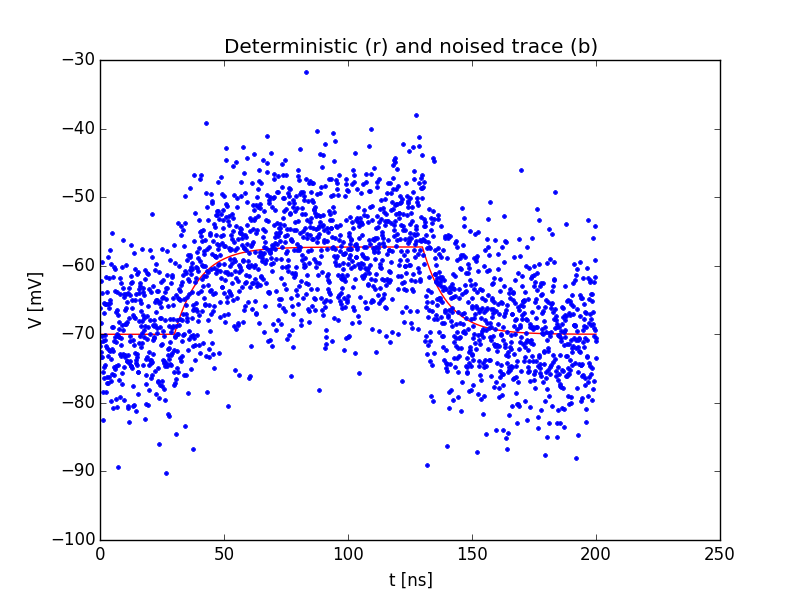
\includegraphics[width=0.49\textwidth]{./fig/cn1/noise.png} }}%
	\hfill
	\subfloat[együttes likelihood]{{\includegraphics[width=0.49\textwidth]{./fig/cn1/likelihood.png} }}%
	\hfill
	\vfill
	\subfloat[együttes poszterior]{{\includegraphics[width=0.5\textwidth]{./fig/cn1/posterior.png} }}%
	\hfill
	\subfloat[$cm$ poszterior]{{\includegraphics[width=0.5\textwidth]{./fig/cn1/cm_posterior.png} }}%
	\caption[Egykompartmentum, színes zaj, két paraméter inferencia]{Az első képen a zaj látható, majd az együttes eloszlások, végül pedig a kimarginalizált $gpas$-al kapott $cm$ poszterior eloszlás.}%
	\label{fig:cn1}
\end{figure}

\begin{figure}
	\hfill
	\subfloat[(A) pont]{{\includegraphics[width=0.49\textwidth]{./fig/cn1/dist100.png} }}%
	\hfill
	\subfloat[(C) pont]{{\includegraphics[width=0.49\textwidth]{./fig/cn1/p_times100.png} }}%
	\hfill
	\vfill
	\subfloat[(E) pont]{{\includegraphics[width=0.5\textwidth]{./fig/cn1/sharp_times100.png} }}%
	\caption[Egykompartmentumos, színes zaj, két paraméter statisztika]{Az első három képen sorban az (A)(C)(E) statisztikák szemléltetése látható.}%
	\label{fig:cn1-stat}
\end{figure}

\FloatBarrier
\subsubsection{Térbelileg kiterjedt modell két változóval}
A kétkompartmentumos modellünk passzív paramétereinek az inferenciáját is elvégeztük színes zajmodell mellett is. $Ra$ paraméter poszterior eloszlására vagyunk kíváncsiak $gpas$ paraméter mellett. Egy eredmény látható a \ref{fig:cn2} ábrán. Ezen a kísérleti protokollon végzett paraméterbecslés pontatlanabb volt az eddigiektől, ez látható a következő adatokon és azok szemléltető \ref{fig:cn2-stat} ábráján.

\begin{verbatim}
(A) A becsült paraméter igazitól való távolsága átlagban: 9.22 (0.09)
(B) Az előbbi érték szórása: 6.5 (0.065)
(C) A poszterior eloszlás maximuma (becsült paraméter), 
hányszorosa az igazi értékhez tartozó valószínűségnek átlagban: 1.25
(D) Az előbbi érték szórása: 0.34
(E) A poszterior eloszlás hányszor élesebb a prior eloszlásnál átlagban: 1.12
(F) A felső érték szórása: 0.03
\end{verbatim}

A zárójelben levő értékek le vannak osztva a paraméter nagyságrendjével, így összehasonlítható a $cm$ paraméterhez kapott eredményekkel. Az eredmények egybevágnak: a poszterior eloszlásom kevésbé éles, ennek következtében viszont ritkábban történhet rossz becslés, amikor a haranggörbe alakú eloszlásom elhagyja az eredeti értéket. 

\begin{figure}
	\hfill
	\subfloat[együttes likelihood]{{\includegraphics[width=0.49\textwidth]{./fig/cn2/likelihood.png} }}%
	\hfill
	\subfloat[együttes poszterior]{{\includegraphics[width=0.49\textwidth]{./fig/cn2/posterior.png} }}%
	\hfill
	\vfill
	\subfloat[$Ra$ poszterior]{{\includegraphics[width=0.5\textwidth]{./fig/cn2/Ra_posterior.png} }}%
	\caption[Kétkompartmentum, színes zaj, két paraméter inferencia]{Az első két képen az együttes eloszlások, végül pedig a kimarginalizált $gpas$-al kapott $Ra$ poszterior eloszlás láthatóak. Az együttes likelihood eloszlás alakjából kivehető, hogy a két paraméter között korreláció van.}%
	\label{fig:cn2}
\end{figure}

\begin{figure}
	\hfill
	\subfloat[(A) pont]{{\includegraphics[width=0.49\textwidth]{./fig/cn2/dist100.png} }}%
	\hfill
	\subfloat[(C) pont]{{\includegraphics[width=0.49\textwidth]{./fig/cn2/p_times100.png} }}%
	\hfill
	\vfill
	\subfloat[(E) pont]{{\includegraphics[width=0.5\textwidth]{./fig/cn2/sharp_times100.png} }}%
	\caption[Kétkompartmentumos, színes zaj, két paraméter statisztika]{Az első három képen sorban az (A)(C)(E) statisztikák szemléltetése látható.}%
	\label{fig:cn2-stat}
\end{figure}








\FloatBarrier
\subsection{Valós kísérleti adatsor}
Valós idegsejt áramimpulzus és áramlépcsőlépcső bemenetre adott feszültségválaszát vizsgálták. A kísérleti eredmény ábrázolása a \ref{fig:compare}-ábrán látható. Ezután a sejtről egy részletes három dimenziós rekonstrukciót készítettek. Ezt a modellt betöltve a Neuron programba és elkészítve hozzá a protokollt (sejtbe injektált áramok a megfelelő időpontokban) majdnem minden megvan a paraméterbecsléses módszerünkhöz. Egyedül a kísérleti zaj autokorrelációs függvénye hiányzik, amiből aztán a kovariancia mátrix megalkotható. Mi jelen esetben sima fehér zajjal közelítve végeztük a becslést. Az eredmények a~\ref{fig:exp} ábrán láthatók.
Előre lefuttatott paraméteroptimalizációs algoritmusok révén már előre tudtuk, hogy milyen tartományokon kell keresni, így ennek megfelelően állítottuk be a paraméterek tartományait. Most is az $Ra$ és $gpas$ paramétereket vettük változóknak. Fontos kiemelni ismét, hogy míg optimalizációval csupán a legjobban illeszkedő paramétereket határoztuk meg (de annak megbízhatóságáról nem nyertünk információt), addig a mi inferenciánk egy teljes poszterior eloszlást biztosít (a kísérleti adatokon alapulva) a paramétertér fölött. Láthatóan a módszer ilyen nagy (valós sejteken alapuló) modellek esetén is megállja a helyét. (A \ref{fig:morph} ábra a modell vetületi képe.)

\begin{figure}
	\hfill
	\subfloat[együttes likelihood]{{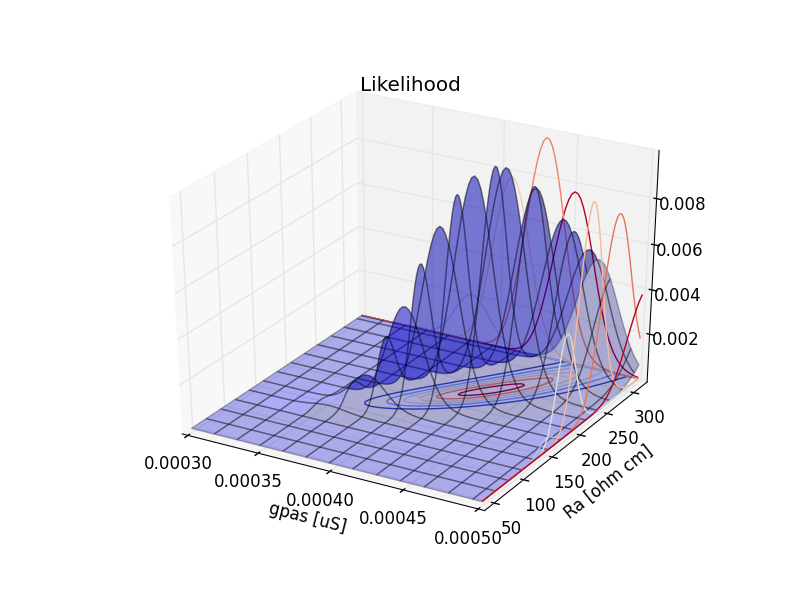
\includegraphics[width=0.49\textwidth]{./fig/exp/likelihood100.png} }}%
	\hfill
	\subfloat[együttes poszterior]{{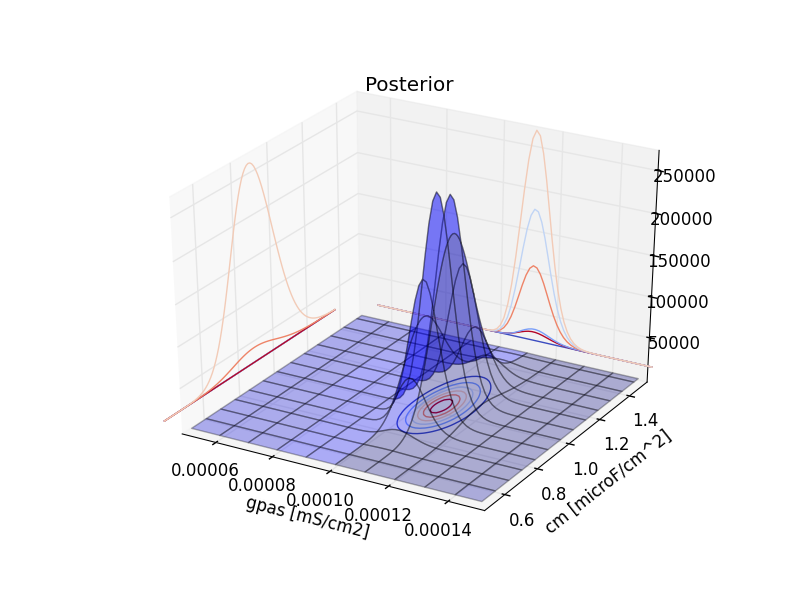
\includegraphics[width=0.49\textwidth]{./fig/exp/posterior100.png} }}%
	\hfill
	\vfill
	\subfloat[$Ra$ poszterior]{{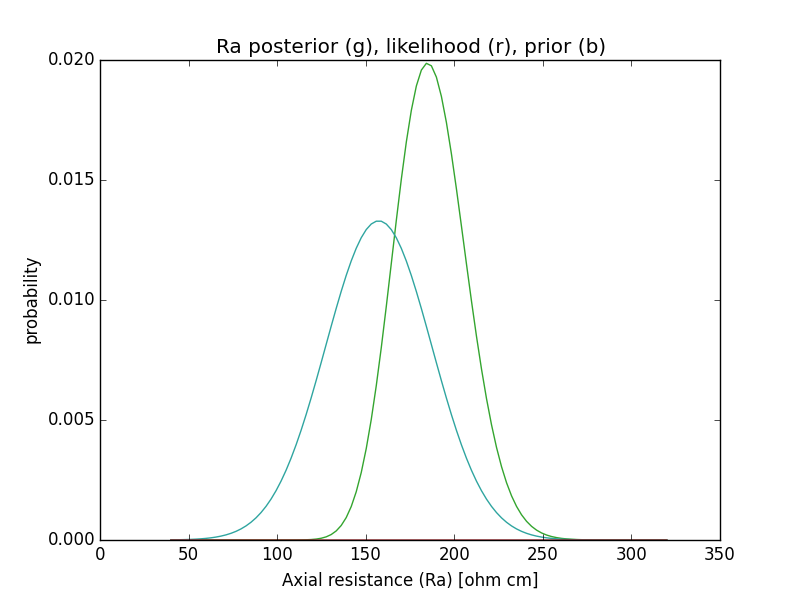
\includegraphics[width=0.5\textwidth]{./fig/exp/Ra_posterior100.png} }}%
	\caption[Kísérleti adatok fehér zajjal közelítve]{Az első két képen az együttes eloszlások, végül pedig a kimarginalizált $gpas$-al kapott $Ra$ poszterior eloszlás láthatóak. Az együttes likelihood eloszlás alakjából kivehető, hogy a két paraméter között korreláció van.}%
	\label{fig:exp}
\end{figure}


